% !TeX encoding = UTF-8
% !TeX root = choix_extensions.tex
\chapter{Mise en page et titres}
\label{ch:miseEnPage}





\section{Choix de la fonte}



\subsection{Quelques informations}
\begin{itemize}
	\item \XeLaTeX \ est notamment conçu pour pouvoir utiliser les fontes Open Type (\incmd{.otf}), True Type (\incmd{.ttf}) et Apple Advance Typogaphy (\incmd{.aat}) du système sur lequel on travaille. Étonnamment, si \XeLaTeX \ voit les fontes du système, il ne voit pas forcément celles de \TeX \ Live sans configuration supplémentaire\dots
	
	\item Dans \LaTeX, les fontes ont quatre paramètres :
	\begin{enumerate}
		\item la famille de fontes : avec empattement, sans empattement, à chasse fixe, mathématique;
		\item la série : la quantité de graisse;
		\item la forme : droite, penchée, italique, en petite capitale;
		\item le corps : la taille de la fonte.
	\end{enumerate}
	\item Les bonnes fontes sont livrées avec une italique redessinée (qui n'est pas une simple version penchée), avec une petite capitale redessinée (qui n'est pas une capitale d'un autre corps), avec une italique grasse et avec toute une série de ligatures.
\end{itemize}



\subsection{Fonte du système}

On peut regarder le nom d'une fonte dans un autre logiciel, p. ex. avec LibreOffice, ou avec le gestionnaire de fonte. Puis on choisit cette fonte avec l'une des commandes : 

\begin{itemize}
	\item \mintinline{latex}{\setmainfont{nom de la fonte}} ou souvent \mintinline{latex}{\setromanfont} pour la fonte romaine de base;
	\item \mintinline{latex}{\setsansfont{nom de la fonte}} pour la fonte sans empattement;
	\item \mintinline{latex}{\setmonofont{nom de la fonte}} pour la fonte à chasse fixe;
	\item \mintinline{latex}{\setmathfont{nom de la fonte}} pour la fonte mathématique.
\end{itemize}

\remarque*{
	Ces commandes sont chatouilleuses : il faut faire attention aux espaces, aux accents, à la casse.
}



\subsection{Fonte \TeX \ Live}
\label{sec:fonteTeXLive}


\subsubsection{Appeler directement les fontes \TeX \ Live}
\TeX \ Live dispose de nombreuses fontes qui se trouvent dans le répertoire de la distribution (p. ex. sous Linux dans \incmd{/usr/local/texlive/2015/texmf-dist/fonts}). On peut accéder aux fontes True Type ou Open Type s'y trouvant en spécifiant leur nom de fichier. Il faut alors spécifier les fichiers correspondant aux différentes séries et formes disponibles (gras, italique, petite capitale, gras italique) si elles existent.

\begin{minted}{latex}
\setmainfont{texgyrepagella-regular.otf}[
  BoldFont=texgyrepagella-bold.otf,
  ItalicFont=texgyrepagella-italic.otf,
  BoldItalicFont=texgyrepagella-bolditalic.otf
]
\setmathfont{texgyrepagella-math.otf}
\end{minted}


\subsubsection{Voir toutes les fontes système disponibles sous Linux}

Pour obtenir la liste des fontes disponibles sous Linux : \lstinline!fc-list :outline -f "%{family}\n" | sort -u!.


\subsubsection{Rendre les fontes de \TeX \ Live visibles par le système}

\attention ceci va faire déferler des hordes de fontes \LaTeX \ Open Type et True Type sur le système. Cette opération dépend du système. Version proposée par ce \href{http://texnique.fr/osqa/questions/115/listes-des-fontes-disponibles}{forum} :
\begin{description}
	\item[Linux] copier le fichier \incmd{/usr/local/texlive/2015/texmf-var/fonts/conf/texlive-fontconfig.conf}, supprimer la ligne se terminant par \incmd{fonts/type1</dir>} et le placer :
	\begin{enumerate}
		\item en tant qu'utilisateur standard : en \incmd{~/.fonts.conf} (si ce fichier existe déjà, il ne faut pas l’écraser, mais fusionner les deux en recopiant les lignes commençant par \incmd{<dir>} du fichier de \TeX \ Live entre \incmd{<fontconfig>} et \incmd{</fontconfig>} dans le fichier existant) puis on lance la commande \incmd{fc-cache};
		\item (si on désire installer ces fontes pour tous les utilisateurs) en tant qu’administrateur : en \newline
		\incmd{/etc/fonts/conf.d/09-texlive.conf} puis on lance la commande \incmd{fc-cache -s}.
	\end{enumerate}
	\item[Mac OS X] ouvrir l’application Livre des fontes puis le menu Fichier → Nouvelle bibliothèque pour créer une nouvelle bibliothèque nommée par exemple \incmd{TeX Live}, qu’on sélectionne ensuite. On ouvre alors le menu \incmd{Fichier} \textrightarrow \incmd{Ajouter des fontes} et, dans la boîte qui apparaît, on utilise le raccourci \incmd{Maj + Cmd + G} pour aller dans le dossier \incmd{/usr/local/texlive/2015/texmf-dist/fonts} où on sélectionne les répertoires opentype et truetype avant de valider.
	\item[Windows] Il n’y a rien à faire, l’installateur \TeX \ Live s’est occupé de tout.
\end{description}



\subsection{Fonte mathématique}

Il n'y a que peu de fontes Open Type Math complètes et qui se comportent gentiment et poliment avec les accents : Latin Modern Math, XITS Math, STIX Math, Asana Math, TeX Gyre Pagella Math\footnote{Il y a aussi d'autres fontes de TeX Gyre qui ont une version Math : Bonum Math, Schola Math, Termes Math (à essayer et bien vérifier avant d'adopter).}.

Pour changer de fonte mathématique, il faut encore faire attention à la cohérence entre les nombres utilisés dans les zones mathématiques et les zones gérées par \incmd{siunitx}. Par exemple, si on veut une fonte Linux Libertine pour le texte et une fonte Pagella Math pour les maths :


\subsubsection{Variante A : les fontes \TeX \ Live sont connues du système}
\begin{minted}{latex}
%
% Pour la fonte de texte
%
\defaultfontfeatures{Scale=MatchLowercase,Ligatures=TeX,Mapping=tex−text}
\setmainfont{Linux Libertine}
%
% Pour la fonte mathématique et les nombres du texte
%
\unimathsetup{math-style=ISO}
\setmathfont{TeX Gyre Pagella Math}[Scale=MatchLowercase]
\newfontfamily\pagellaM[Numbers=Lining]{TeX Gyre Pagella Math}
\sisetup{mode = text,number-text-rm = \pagellaM}
\end{minted}

Avec ça, les nombres dans les parties mathématiques et dans les parties gérées par \incmd{siunitx} sont en Pagella. Les nombres dans les parties texte restent en Libertine\footnote{Ca n'a pas l'air franchement évident de faire en sorte que tous les nombres soient les mêmes. En cas de besoin, mieux vaut utiliser \inlatex{\num{1234}} pour mettre 1234 en fonte mathématique.}.


\subsubsection{Variante B : les fontes \TeX \ Live ne sont pas vues par le système}
\begin{minted}{latex}
%
% Pour la fonte de texte
%
\defaultfontfeatures{Scale=MatchLowercase,Ligatures=TeX,Mapping=tex−text}
%\setmainfont{Linux Libertine}
%\setmonofont{Linux Libertine Mono}[Scale=MatchLowercase]
%\setsansfont{Linux Biolinum}[Scale=MatchLowercase]
\setmainfont{LinLibertine_R.otf}[
		BoldFont=LinLibertine_RB.otf,
		ItalicFont=LinLibertine_RI.otf,
		BoldItalicFont=LinLibertine_RBI.otf	
	]
\setmonofont{LinLibertine_M.otf}[Scale=MatchLowercase]
\setsansfont{LinBiolinum_R.otf}[Scale=MatchLowercase]
%
% Pour la fonte mathématique
%
\unimathsetup{math-style=ISO}
\setmathfont{texgyrepagella-math.otf}[Scale=MatchLowercase]
\newfontfamily\pagellaM[Numbers=Lining]{texgyrepagella-math.otf}
\sisetup{mode = text,number-text-rm = \pagellaM}
\end{minted}


\subsection{Fontes supplémentaires}

Question de base : est-ce vraiment une si bonne idée ? Si oui\dots


\subsubsection{Fontes non libres de \TeX \ Live}

Pour installer les fontes non libres de \TeX \ Live \url{http://www.tug.org/fonts/getnonfreefonts/}.


\subsubsection{Quelques ressources}

\begin{itemize}
	\item Exemples :
		\href{http://www.math.ucsd.edu/~msharpe/ffsamples.pdf}{ffsamples.pdf},
		\href{http://www.tug.org/fonts/special-s.pdf}{\TeX \ font sampler} (voir les informations à la fin du document);
	\item Identifier des fontes :
		\href{http://www.identifont.com/similar.html}{Identifon};
	\item Liste des fontes de \TeX Live
		\href{https://www.ctan.org/topic/font-otf}{Open Type}
			\footnote{\label{foot:fontePackage} \attention il ne faut pas appeler l'extension correspondante, mais seulement la fonte en question, selon le mécanisme décrit dans \ref{sec:fonteTeXLive}.},
		\href{https://www.ctan.org/topic/font-ttf}{True Type}\footref{foot:fontePackage}, et
		\href{https://www.ctan.org/topic/font-maths}{mathématiques},
		\href{http://www.tug.dk/FontCatalogue/}{The \LaTeX \ Font Catalogue} (toutes les fontes);
	\item Fonderies et dépôts libres :
		\href{http://www.sil.org/resources/software_fonts}{SIL}, \href{http://www.gust.org.pl/projects/e-foundry/tex-gyre/}{TeX Gyre},
		\href{http://www.fontsquirrel.com}{Font Squirrel},
		\href{http://www.exljbris.com}{exljbris},
		\href{http://delubrum.org/}{Delubrum},
		\href{https://fontlibrary.org/}{Open Font Library},
		\href{http://fontsgeek.com}{fontsgeek.com},
		\href{http://www.dafont.com/fr/}{dafont.com};
	\item Fonderies commerciales :
		\href{http://www.linotype.com/fr/}{Linotype},
		\href{http://www.fontspring.com}{Fontspring},
		\href{http://www.adobe.com/products/type/fonts-by-adobe.html}{Adobe},
		\href{https://typekit.com}{Adobe Typekit}.
\end{itemize}





\section{Gestion des longueurs (length)}
\label{sec:gestionLongueurs}

Parfois, il est nécessaire d'afficher les valeurs numériques de longueurs pour les régler finement. Dans ce cas, l'extension \mintinline{latex}{\usepackage{printlen}} fournit la commande \mintinline{latex}{\printlength} :

\begin{LTXexample}[pos=o]
\printlength{\linewidth}
\end{LTXexample}
 





\section{Page de titre}

La page de titre s'obtient avec l'environnement \mintinline{latex}{\begin{titlepage}} :
	
\vspace{1em}
\begin{minipage}{.48\linewidth}
	\begin{minted}{latex}
\documentclass[twoside]{report}
\usepackage[a6paper]{geometry}
\usepackage{titlesec}
\usepackage[latin1]{inputenc}
\usepackage{ccicons}

\begin{document}
  \begin{titlepage}
    \vspace{5cm}
    \centerline{\Huge{Géométrie première}}
    \vspace{.3cm}
    \centerline{\LARGE Support de cours}
    \vspace{7cm}
    \centerline{Commission de géométrie}
    \centerline{Version 2011-2012}
    \centerline{
    \ccLogo \ccAttribution
    \ccNonCommercialEU \ccShareAlike
  }
  \end{titlepage}
\end{document}
	\end{minted}
\end{minipage}
\hfill
\begin{boxedminipage}{.4\linewidth}
	\centering
	
\includegraphics[scale=.5]{images/choix_extensions_exemple_titlePage}
\end{boxedminipage}
	
	
	
	

\section{Personnalisation des titres}



\subsection{Apparence des titres}

Les titres de chapitres, sections\dots \ peuvent être personnalisés grâce à l'extension \href{http://mirror.ctan.org/macros/latex/contrib/titlesec/titlesec.pdf}{titlesec}. Par exemple, les titres de chapitre de ce document sont définis dans \incmd{preambule_personalisation.sty} par le code suivant :

\begin{minted}{latex}
\titleformat{\chapter}[frame]        % frame pour avoir un cadre
    {\normalfont\small\scshape}      % Format du bandeau
    {\ Chapitre \thechapter\ }       % Texte du bandeau
    {.5cm}              % avec frame : esp. vertical autour du titre
    {\LARGE\bfseries\filcenter}[]    % avant la composition du titre

\titlespacing{\chapter} % régler l'espacement autour du titre de chapitre
    {0pt}   % à gauche
    {-1cm}  % avant
    {1cm}   % après
    [0pt]   % à droite
\end{minted}

Pour plus de souplesse, notamment pour pouvoir changer de style entre les chapitres normaux et ceux de l'annexe, ce code a été introduit dans une commande : \mintinline{latex}{\newcommand{\chapterFormat}{...}}. Cette commande est appelée dans le fichier principal de ce document (\mintinline{latex}{choix_extensions.tex}).



\subsection{Numérotation des titres}

Si on veut éviter que les titres de sections reprennent le numéro du chapitre en cours, il faut dé-commenter la ligne suivante dans \incmd{preambule_personalisation.sty} : \mintinline{latex}{\renewcommand{\thesection}{\arabic{section}}}. Il est aussi possible d'insérer cette commande en cours de document.





\newpage






\section{Interligne}

Pour régler l'interligne avec l'extension \href{http://ctan.org/pkg/setspace}{setspace} : en utilisant les commandes \mintinline{latex}{\singlespacing}, \mintinline{latex}{\onehalfspacing}, et \mintinline{latex}{\doublespacing}. Par exemple : 
\begin{LTXexample}[pos=o,width=.5]
\onehalfspacing
Donec in nisl. Fusce vitae est. Vivamus ante ante, mattis laoreet, posuere eget, congue vel, nunc. Fusce sem. Nam vel orci eu eros viverra luctus. Pellentesque sit amet augue. Nunc sit amet ipsum et lacus varius nonummy.
\end{LTXexample}

On obtient le même effet pour l'ensemble du document avec les options : \mintinline{latex}{singlespacing}, \mintinline{latex}{onehalfspacing} et \mintinline{latex}{doublespacing}. Par exemple avec \mintinline{latex}{\usepackage[onehalfspacing]{setspace}}.





\section{En-tête et pied de page personnalisés}

À faire avec l'extension \href{http://mirror.ctan.org/macros/latex/contrib/fancyhdr/fancyhdr.pdf}{fancyhdr}. Par exemple, \incmd{preambule_personnalisation.sty} du présent document contient :

\begin{minted}{latex}
\pagestyle{fancy}
\renewcommand{\chaptermark}[1]{\markboth{\thechapter. \ #1}{}}
\renewcommand{\sectionmark}[1]{\markright{\thesection\ #1}}
\fancyhf{}
\fancyhead[LO,RE]{\bfseries \rightmark}
\fancyhead[LE,RO]{\bfseries \leftmark}
\fancyfoot[C]{\thepage}
\fancypagestyle{plain}{
    \fancyhead{}
    \renewcommand{\headrulewidth}{0pt}
    \fancyfoot[C]{\thepage}
}
\setlength\headheight{15pt}
\end{minted}





\section{Table des matières par chapitre}

Avec l'extension \href{http://mirror.ctan.org/macros/latex/contrib/minitoc/minitoc-fr.pdf}{\mintinline{latex}{minitoc}}. Attention, actuellement, il est commenté dans le fichier \incmd{preambule_college.sty}. Sans cela, il interfère et génère une page vide à la fin du document\dots

\begin{itemize}
	\item Dans le préambule : placer \mintinline{latex}{\dominitoc[n]} et soit \mintinline{latex}{\tableofcontents}, soit \mintinline{latex}{\faketableofcontents} si on ne veut pas de table globale.
	\item Dans le document : insérer \mintinline{latex}{\minitoc} où l'on veut la table.
\end{itemize}

\begin{minipage}{.48\linewidth}
	\begin{minted}{latex}
\documentclass[a4paper,twoside]{report}
\usepackage{minitoc}
\dominitoc[n]
\faketableofcontents
\begin{document}
\chapter{Mon chapitre}
\section{Dans ce chapitre}
\minitoc
\section{Ma section 1}
\subsection{Ma section 1}
    bla bla
\section{Ma section 2}
    bla bla
\end{document}
	\end{minted}
\end{minipage}
\hfill
\begin{boxedminipage}{.4\linewidth}
	\centering
	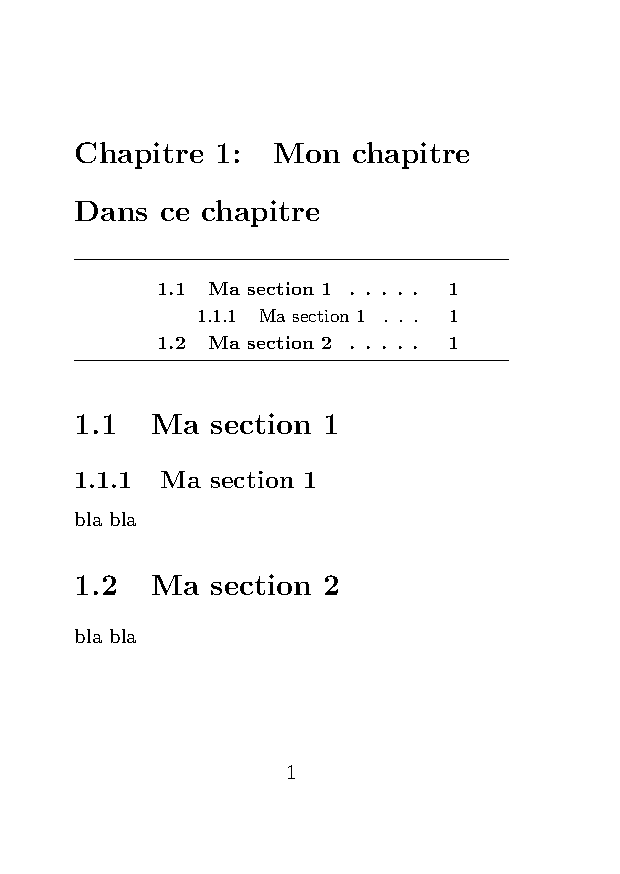
\includegraphics[scale=.5]{images/choix_extensions_exemple_minitoc}
\end{boxedminipage}





\section{Boîte autour d'une minipage}
Avec l'extension \href{http://mirror.ctan.org/macros/latex/contrib/boxedminipage/boxedminipage.pdf}{boxedminipage} (documentation plutôt sommaire !) :
\begin{LTXexample}[pos=o,width=.4]
\begin{boxedminipage}[t]{3cm}
    Voyez le brick géant que j'examine près du wharf.
\end{boxedminipage}
\begin{boxedminipage}[t]{3cm}
    Quel beau bateau\dots
\end{boxedminipage}
\end{LTXexample}




\section{Composition en colonne}



\subsection{En cours de document}

Utiliser \mintinline{latex}{\multicols} :

\begin{LTXexample}[pos=o]
    \begin{multicols}{2}
        Premier paragraphe
		
        Deuxième paragraphe
    \end{multicols}
\end{LTXexample}



\subsection{Pour tout un document}

On peut composer tout un document en deux colonnes en utilisant les options \mintinline{latex}{twocolomn} et \mintinline{latex}{columnsep} de l'extension \mintinline{latex}{geometry}, par exemple \mintinline{latex}{\usepackage[twocolumn,columnsep=2cm]{geometry}} :

\vspace{1em}
\begin{minipage}{.48\linewidth}
    \begin{minted}{latex}
    \documentclass{report}
    \usepackage[twocolumn,columnsep=2cm,
        a6paper]{geometry}
    \usepackage{lipsum}
    \begin{document}
         \lipsum[1]
    \end{document}
    \end{minted}
\end{minipage}
\begin{boxedminipage}{.48\linewidth}
	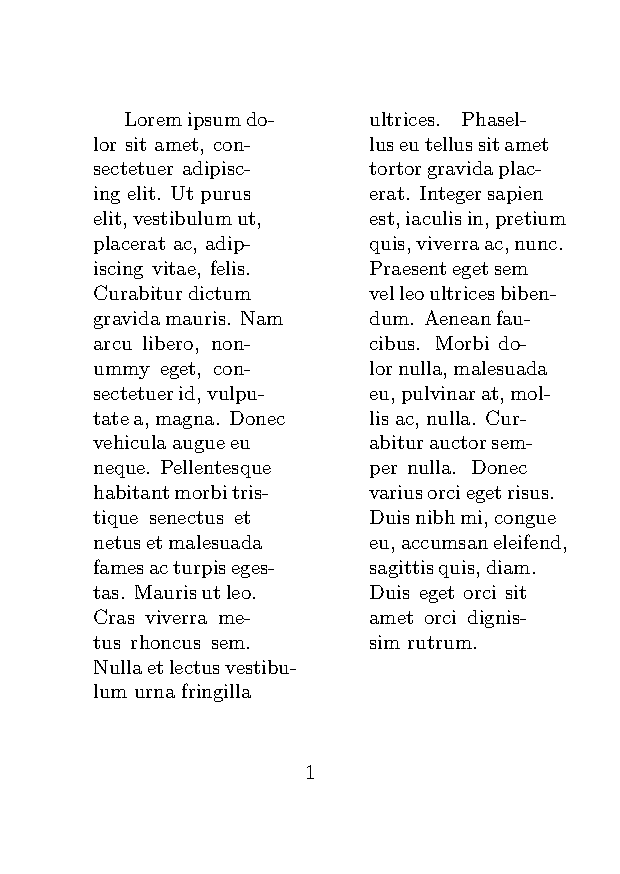
\includegraphics[scale=.6]{images/choix_extensions_exemple_colonnes}
\end{boxedminipage}





\section{Composition à l'italienne (landscape)}



\subsection{En cours de document}

Avec l'extension \mintinline{latex}{lscape} : placer le contenu de la page à l'italienne dans l'environnement \mintinline{latex}{landscape}. Dans ce cas, l'en-tête et le pied de page restent en place comme dans :

\vspace*{1em}
\begin{minipage}{.48\linewidth}
    \begin{minted}{latex}
    \documentclass{report}
    \usepackage[a6paper]{geometry}
    \usepackage{lscape}
    \usepackage{lipsum}
    \begin{document}
    \begin{landscape}
    \section*{A l'italienne}
         \lipsum[1]
    \end{landscape}
    \end{document}
    \end{minted}
\end{minipage}
\begin{boxedminipage}{.48\linewidth}
	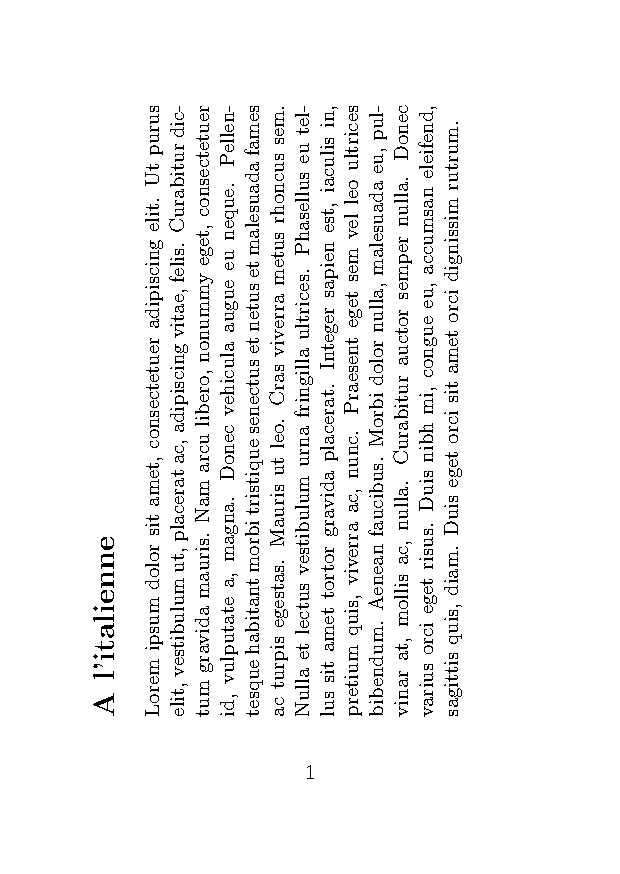
\includegraphics[width=\linewidth]{images/choix_extensions_exemple_lscape}
\end{boxedminipage}



\subsection{Pour tout un document}

Utiliser l'option \mintinline{latex}{landscape} dans l'extension \mintinline{latex}{geometry} : \mintinline{latex}{usepackage[landscape]geometry} :

\vspace{1em}
\begin{minipage}{.48\linewidth}
	\begin{minted}{latex}
    \documentclass{report}
    \usepackage[landscape,a6paper]
         {geometry}
    \usepackage{lipsum}
    \begin{document}
    \lipsum[47]
    \end{document}
	\end{minted}
\end{minipage}
\begin{boxedminipage}{.48\linewidth}
	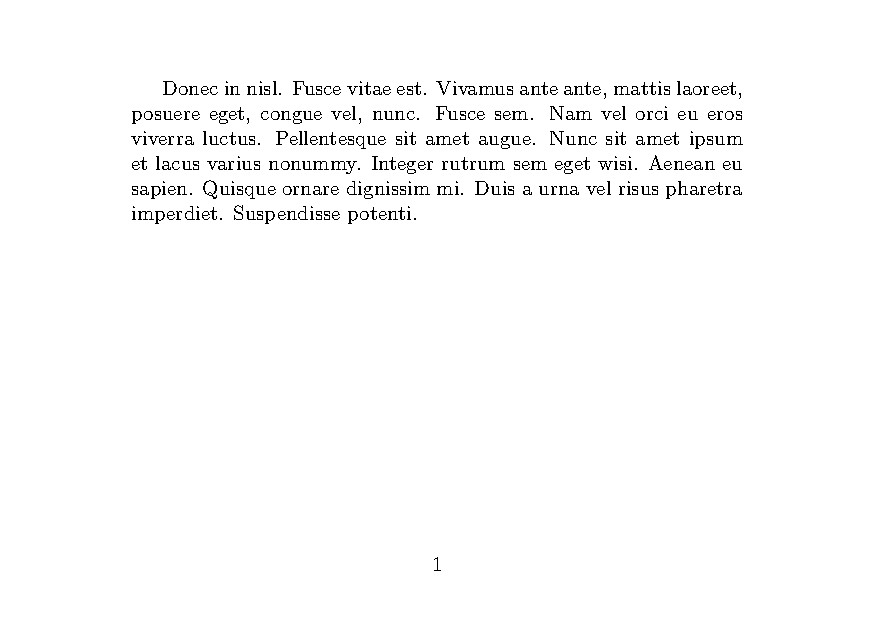
\includegraphics[width=\linewidth]{images/choix_extensions_exemple_landscape}
\end{boxedminipage}






\section{Imprimer en A5}

La gestion du A5 dépend plus de l'imprimante et de ses pilotes que de \LaTeX.

Si l'imprimante support du papier au format A5 : utiliser l'extension \href{}{geometry} avec l'option a5paper : \newline \mintinline{latex}{\usepackage[a5paper]{geometry}}. Ceci génère un PDF au format A5.

Sinon, on peut :
\begin{itemize}
	\item soit garder l'option ci-dessus et, si le driver de l'imprimante le permet, faire tirer deux pages par feuille sans réduction de taille;
	\item soit, ce qui est plus courant, créer des documents en A4 et faire tirer deux pages sur une. Attention à la réduction de taille d'environ \SI{71}{\%} (les fontes en \SI{12}{pt} ressortent environ en \SI{8,5}{pt}).
\end{itemize}